\documentclass[11pt,reqno]{amsart}

\usepackage[margin=0.95in]{geometry}
\usepackage{amsmath,amssymb,amsthm}
\usepackage{booktabs}
\usepackage{tabularx}
\usepackage{array}
\usepackage{graphicx}
\usepackage{xcolor}
\usepackage{enumitem}
\usepackage{microtype}
\usepackage{placeins}
\usepackage{xurl}
\usepackage[hidelinks,colorlinks=true,linkcolor=blue!60!black,citecolor=teal!70!black,urlcolor=blue!70!black]{hyperref}

\theoremstyle{plain}
\newtheorem{theorem}{Theorem}[section]
\newtheorem{proposition}[theorem]{Proposition}
\theoremstyle{definition}
\newtheorem{definition}[theorem]{Definition}
\newtheorem{remark}[theorem]{Remark}

\newcolumntype{Y}{>{\raggedright\arraybackslash}X}
\newcolumntype{P}[1]{>{\raggedright\arraybackslash}p{#1}}
\newcommand{\code}[1]{{\footnotesize\nolinkurl{#1}}}
\newcommand{\tcode}[1]{{\scriptsize\nolinkurl{#1}}}
\newcommand{\tagkc}{\textsc{kernel-checked}}
\newcommand{\tagpa}{\textsc{program-audited}}
\newcommand{\tagri}{\textsc{registry-indexed}}
\newcommand{\tagee}{\textsc{editorial-est.}}
\newcommand{\tagoc}{\textsc{open-conj.}}

\title[Unsolved Problems Mega-Atlas (V2.4.0)]{Unsolved Problems Mega-Atlas (V2.4.0): A Multi-Layer Taxonomy, Biconnected Knowledge Graph, Six-Kernel Lean 4.35.0 Formal Invariant Suite, and Deterministic Research Infrastructure Across 1,900 Open Problems}

\author{Alexander Stephen Donahue}
\address{Independent Researcher, Spokane, WA, USA}
\email{0\_0@0thernes.art}
\urladdr{https://orcid.org/0009-0006-8168-9648}

\date{November 25, 2026}
\subjclass[2020]{Primary 03B35, 68T30; Secondary 05C90, 68P20}
\keywords{open problems, knowledge graph, Lean 4, multi-kernel formal verification, RAG, MCP, FAIR metadata, AutoResearch}

\begin{document}

\begin{abstract}
No single fixed count of open scientific or mathematical problems exists, and rapid Fall--November 2026 AI proof announcements have created a sharp divide between machine-checked formal compilation, statement fidelity, human exposition, and community consensus. We present Version~2.4.0 of the \emph{Unsolved Problems Mega-Atlas}, an open-source, strictly deduplicated research infrastructure cataloging $1{,}900$ unsolved, open, and hard problems spanning $8$ Macro-Pillars, $28$ Superdomains, $8$ physical/formal Substrates, $7$ Abstraction Layers ($\text{L0}$--$\text{L6}$), and $1{,}752$ subdomains, wired into a single biconnected $5{,}808$-edge knowledge graph ($0$ articulation points, $0$ bridges, $0$ dangling links, $35.7\%$ cross-superdomain, $18.7\%$ cross-pillar).

To separate exact mathematical invariants from editorial judgment, we pair the dataset with: (i) a zero-Mathlib \emph{Lean~4.35.0} formal invariant suite of $92$ audited theorems ($72$ core module invariants, $12$ concrete non-vacuity and negative-boundary witnesses, and $8$ Palomar comparator specifications) verified across six independent proof kernels (\code{lean}, \code{leanchecker-paranoid}, \code{lean4lean}, \code{nanoda_bin}, \code{con-leche}, and \code{con-ron}) using constructive axioms strictly within [\code{propext}, \code{Quot.sound}]; (ii) a $50$-digit \code{Decimal}/\code{Fraction} reference oracle differentially verifying the Python scoring pipeline across $2{,}000+$ cases plus $100\%$ ($6/6$) mutation-kill coverage; (iii) a deterministic offline SQLite FTS5 hybrid BM25 + bigram + PageRank RAG engine achieving $100.0\%$ MRR@5 ($25/25$ top-1) exposed via a zero-dependency $10$-tool Model Context Protocol (MCP) server; and (iv) an immutable Karpathy-style AutoResearch harness (\code{AQS} $= 97.99$) alongside a finite arbitrary-precision Track~B Antihydra probe (\code{LOG-002}).

\emph{Honest verification boundary:} Our Lean~4 theorems verify scoring, taxonomy, graph handshaking, deduplication, AutoResearch ratchet, and margin invariants \emph{only}. Zero ($0 / 1{,}900$) overarching Mega-Atlas open problems are claimed solved or retired. Quantitative rubric inputs are disclosed AI-assisted editorial estimates, not peer-reviewed empirical measurements.
\end{abstract}

\maketitle

\section{Introduction and the November 25, 2026 Verification Landscape}
\label{sec:intro}

Cataloging the frontier of unsolved human inquiry faces two structural challenges. First, open-problem trackers are deeply siloed by discipline: mathematical registries such as ProofAtlas~\cite{proofatlas2026} ($1{,}100+$ eligible problems; $243$ open in the Top-500 subset), the Erd\H{o}s Problems Database~\cite{bloom_erdos} ($\sim 1{,}221$ tracked; $\sim 630$ open), and the Clay Millennium Prize list~\cite{clay2000} rarely connect formally to open frontiers in condensed matter, origin of life, consciousness, post-Moore silicon, climate sensitivity, or normative ethics. Second, during September--November 2026, rapid frontier AI proof announcements---including OpenAI's September~8 3D Navier--Stokes claim, OpenAI's October~6 bulk dump of $722$ unrefereed manuscripts across $372$ topics, and the November~20--21 multi-kernel Lean certification of the Alp\"oge/Claude $\sim 17\text{M}$-line Riemann Hypothesis and GRH archive (with no complete human-readable proof paper yet, alongside Stanford's Masullo human draft under gap scrutiny)---demonstrated that kernel compilation alone is insufficient for community retirement of a conjecture.

\begin{figure}[t]
  \centering
  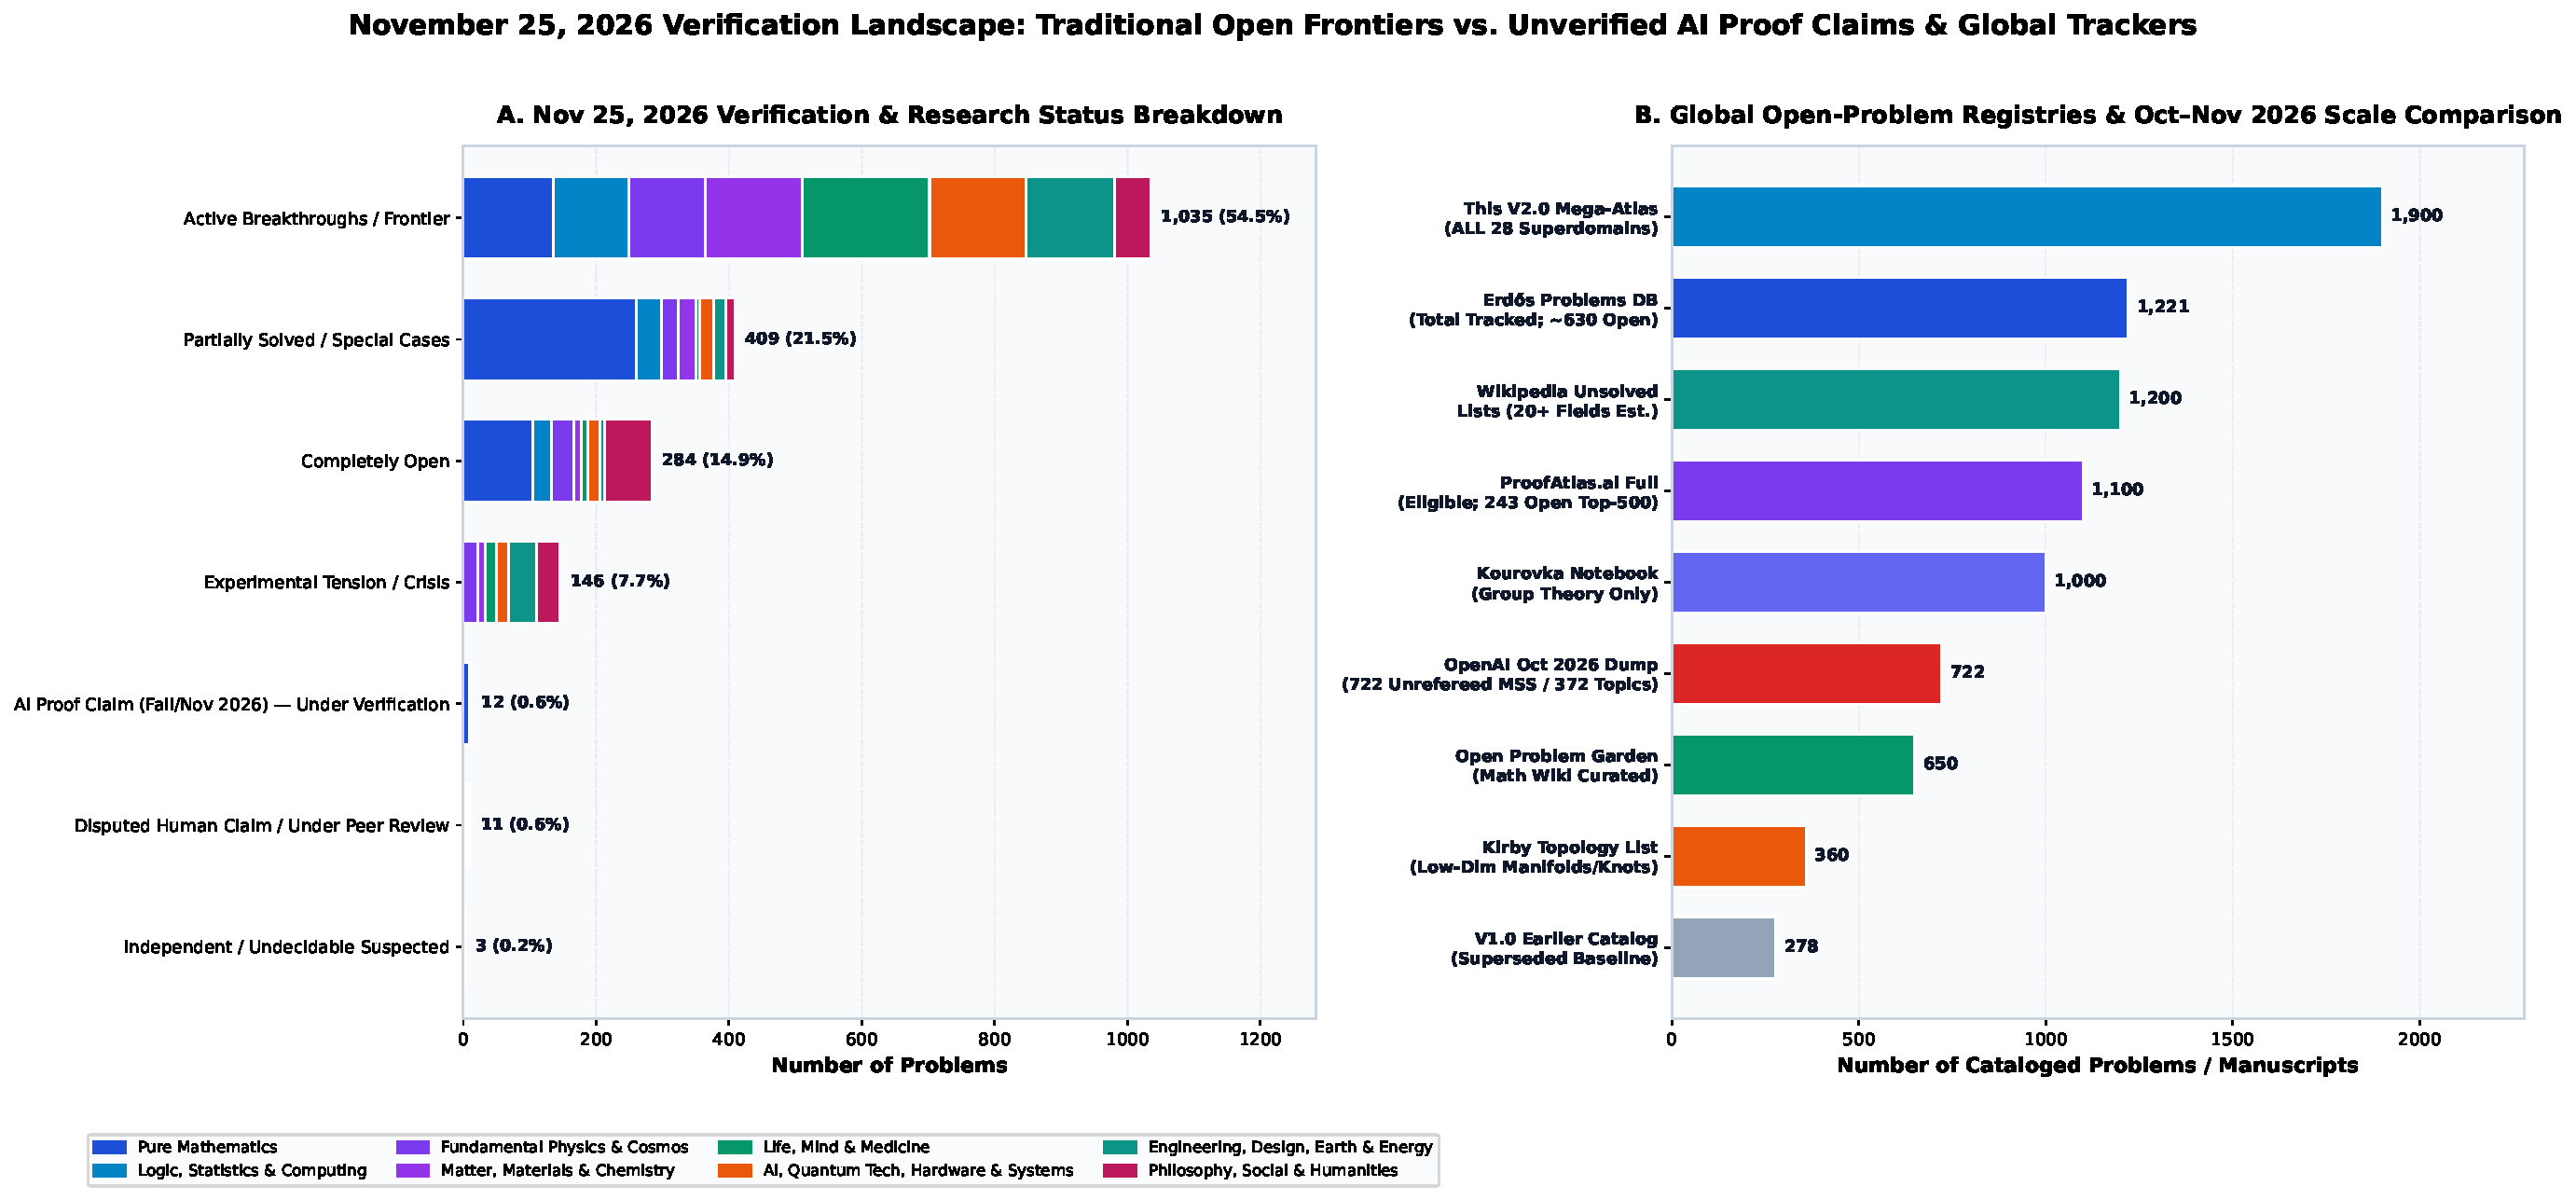
\includegraphics[width=0.95\textwidth]{figures/fig11_nov2026_status.pdf}
  \caption{November 25, 2026 verification landscape: distribution of research statuses across the $1{,}900$-problem Mega-Atlas (left) and scale comparison against $13$ global open-problem trackers and Fall 2026 AI claim dumps (right). All $12$ Fall/November 2026 AI proof-claim targets remain flagged \code{ai-claim-under-audit-nov2026} and officially unretired.}
  \label{fig:nov2026}
\end{figure}

Figure~\ref{fig:nov2026} summarizes the November~25, 2026 status distribution and compares this atlas against $13$ major registries. Rather than declaring volatile AI claims resolved, the Mega-Atlas preserves an explicit per-record provenance field (\code{verification_flag}) separating primary-registry-indexed problems ($925$), AI-assisted editorial syntheses ($952$), November~2026 AI claims under audit ($12$), and disputed human claims ($11$).

\section{Claims Ledger and Epistemic Provenance Architecture}
\label{sec:claims}

Every headline claim in this repository is tagged with one of five epistemic tiers and paired with a concrete verification artifact and explicit refutation condition (Table~\ref{tab:claims}; full command-verified ledger in \code{CLAIMS.md}).

\begin{table}[t]
\centering
\caption{Numbered Claims Ledger separating kernel-checked mathematical invariants from program-audited dataset properties, registry indices, editorial scores, and open conjectures.}
\label{tab:claims}
\scriptsize
\renewcommand{\arraystretch}{1.18}
\begin{tabularx}{\textwidth}{@{}P{0.45cm}P{1.95cm}YP{3.0cm}P{2.55cm}@{}}
\toprule
\textbf{ID} & \textbf{Tier} & \textbf{Exact Claim Statement} & \textbf{Primary Artifact} & \textbf{Refutation Condition} \\
\midrule
C1 & \tagkc & $92$ Pure Lean~4.35.0 theorems (M1--M7 + NonVacuity) compile with $0$ \tcode{sorry} in \tcode{lean/}, axioms $\subseteq$ [\tcode{propext}, \tcode{Quot.sound}], across $6/6$ kernels. & \tcode{lean/}, \tcode{results/lean_axioms.txt} & Any kernel rejects or unpermitted axiom appears. \\
C2 & \tagpa & $1{,}900$ strictly unique records ($48$ JSON-Schema-valid fields) form $1$ biconnected $5{,}808$-edge graph ($0$ APs, $0$ bridges, $0$ dangling links). & \tcode{src/v2_loader.py}, \tcode{scripts/audit_atlas.py} & Duplicate ID, schema error, AP $>0$, or link error. \\
C3 & \tagpa & Python scoring matches $50$-digit \tcode{Decimal}/\tcode{Fraction} oracle across $2{,}000+$ cases ($< 10^{-2}$ rounding) and kills $6/6$ planted mutants. & \tcode{reference/scoring_oracle.py}, \tcode{scripts/run_mutation_audit.py} & Any oracle divergence or surviving mutant. \\
C4 & \tagpa & Offline FTS5 hybrid BM25+bigram+PageRank RAG achieves $100.0\%$ MRR@5 ($25/25$ top-1) and immutable \tcode{AQS} $= 97.99$. & \tcode{rag/query.py}, \tcode{autoresearch/evaluate.py} & MRR@5 $< 100\%$ or hard gate fails. \\
C5 & \tagri & All $12$ Fall/Nov 2026 AI proof claims (\tcode{NT-001}, \tcode{NT-002}, \tcode{ANL-001}, etc.) remain officially unretired at CMI/community registries. & \tcode{src/v2_loader.py} (\tcode{AI_AUDIT}) & Official CMI or journal consensus retirement. \\
C6 & \tagpa & Track~B Antihydra (\tcode{LOG-002}) canonical orbit ($a_0=8$, $5{,}000$ exact bigint steps) does not halt ($b_{5000}=2{,}599$, $\min b = 0$); $66/99$ seeds in $[2,100]$ halt $\le 2{,}000$ steps. & \tcode{research/runs/LOG-002_antihydra_pilot/} & Independent bigint re-execution disagrees. \\
C7 & \tagee & Difficulty, tractability, impact, and interdisciplinarity scores ($1$--$10$) are falsifiable editorial estimates, not peer-reviewed measurements. & \tcode{docs/METHODOLOGY.md}, \tcode{RANKING.md} & N/A (explicitly declared editorial estimate). \\
C8 & \tagoc & Zero ($0/1{,}900$) overarching Mega-Atlas open problems are retired by this repository or by the author's $7$ scoped companion preprints. & \tcode{LIMITATIONS.md}, Section~\ref{sec:author_preprints} & Peer-reviewed proof of an overarching ID. \\
\bottomrule
\end{tabularx}
\end{table}

\section{Multi-Layer Taxonomy, Scoring Metrics, and Biconnected Connectome}
\label{sec:taxonomy}

Each record $p \in \mathcal{P}$ ($|\mathcal{P}| = 1{,}900$, deduplicated from $1{,}912$ authored entries via $12$ audited alias merges) carries $48$ typed fields validated against JSON Schema Draft~2020-12 (\code{schema/problem.schema.json}) and mapped cleanly across four orthogonal structural axes: $8$ Macro-Pillars, $28$ Superdomains (partition $5+3+3+3+3+4+4+3=28$), $8$ physical/formal Substrates, and $7$ Abstraction Layers ($\text{L0}$ Formal/Axiomatic through $\text{L6}$ Normative/Economic/Semantic).

\subsection{Scoring Definitions}
For integer ratings $d, i, r, t \in \{1,\dots,10\}$ (difficulty, civilizational impact, interdisciplinarity, 2050 tractability), graph degree $\deg(p) \in \mathbb{N}$, and frozen 2026 age $a = \max(0, 2026 - y) \in \mathbb{N}$, we define:
\begin{align}
  \mathrm{CSS}(p) &= 0.40\,(10d) + 0.30\,\bigl(5i + \tfrac{1}{2}\min(100, 25\ln(1+\deg(p)))\bigr) \nonumber \\
                  &\quad + 0.20\,\min(100, a/3) + 0.10\,(100 - 10t) \in [5.5, 100], \label{eq:css}\\
  \mathrm{Titan}(p) &= 0.35\,d + 0.35\,i + 0.20\,r + 0.10\,\min(10, 2.5\ln(1+\deg(p))) \in [0.90, 10.00], \label{eq:titan}\\
  \mathrm{Lev}(p) &= \frac{i \cdot t}{10} \in [0.1, 10.0], \qquad
  \Delta_{\mathrm{DT}}(p) = d - t \in [-9, 9]. \label{eq:lev}
\end{align}
The antiquity term $\min(100, a/3)$ saturates at $300$ years so ancient problems do not overwhelm modern structural hardness, while the dual-ranking margin $M_{\mathrm{CT}}(p) = \mathrm{CSS}(p) - 10\,\mathrm{Titan}(p)$ exposes age-heavy foundational enigmas versus cross-disciplinary leverage hubs. Table~\ref{tab:pillars} reports exact aggregate statistics across all $8$ Macro-Pillars; Figures~\ref{fig:superdomains}, \ref{fig:quadrant}, and \ref{fig:substrates} visualize the 28-superdomain profile, strategic 4-quadrant partition ($758$ Q1, $169$ Q2, $393$ Q3, $580$ Q4), and $8 \times 7$ Substrate--Layer reality stack.

\begin{table}[t]
\centering
\caption{Exact quantitative profile across all $8$ Macro-Pillars ($N = 1{,}900$, $|E| = 5{,}808$ biconnected edges, computed by \code{src/v2_loader.py} v2.4.0).}
\label{tab:pillars}
\scriptsize
\setlength{\tabcolsep}{4.5pt}
\renewcommand{\arraystretch}{1.15}
\begin{tabular}{@{}lrrrrrrrrr@{}}
\toprule
\textbf{Macro-Pillar} & \textbf{$N$} & \textbf{Share} & \textbf{SDs} & \textbf{$\bar{d}$} & \textbf{$\bar{t}_{2050}$} & \textbf{$\bar{i}$} & \textbf{$\overline{\mathrm{Titan}}$} & \textbf{$\overline{\mathrm{CSS}}$} & \textbf{XP Edges} \\
\midrule
Pure Mathematics                       & 514 & 27.1\% & 5 & 8.87 & 4.96 & 5.44 & 6.53 & 59.90 & 205 \\
Logic, Statistics \& Computing         & 185 &  9.7\% & 3 & 8.48 & 6.31 & 6.48 & 7.09 & 57.27 & 284 \\
Fundamental Physics \& Cosmos          & 201 & 10.6\% & 3 & 8.11 & 7.18 & 7.33 & 7.40 & 56.47 & 225 \\
Matter, Materials \& Chemistry         & 196 & 10.3\% & 3 & 7.79 & 8.06 & 7.82 & 7.51 & 55.46 & 295 \\
Life, Mind \& Medicine                 & 224 & 11.8\% & 3 & 7.58 & 8.33 & 8.55 & 7.81 & 55.97 & 250 \\
AI, Quantum Tech, Hardware \& Systems  & 203 & 10.7\% & 4 & 7.99 & 7.96 & 8.60 & 7.94 & 55.54 & 372 \\
Engineering, Design, Earth \& Energy   & 202 & 10.6\% & 4 & 7.39 & 8.47 & 8.38 & 7.68 & 54.64 & 286 \\
Philosophy, Social \& Humanities       & 175 &  9.2\% & 3 & 7.75 & 5.77 & 7.83 & 7.71 & 59.90 & 251 \\
\midrule
\textbf{All 8 Macro-Pillars (Total / Mean)} & \textbf{1,900} & \textbf{100.0\%} & \textbf{28} & \textbf{8.13} & \textbf{6.81} & \textbf{7.22} & \textbf{7.31} & \textbf{57.33} & \textbf{1,084 uniq.} \\
\bottomrule
\end{tabular}
\end{table}

\begin{figure}[p]
  \centering
  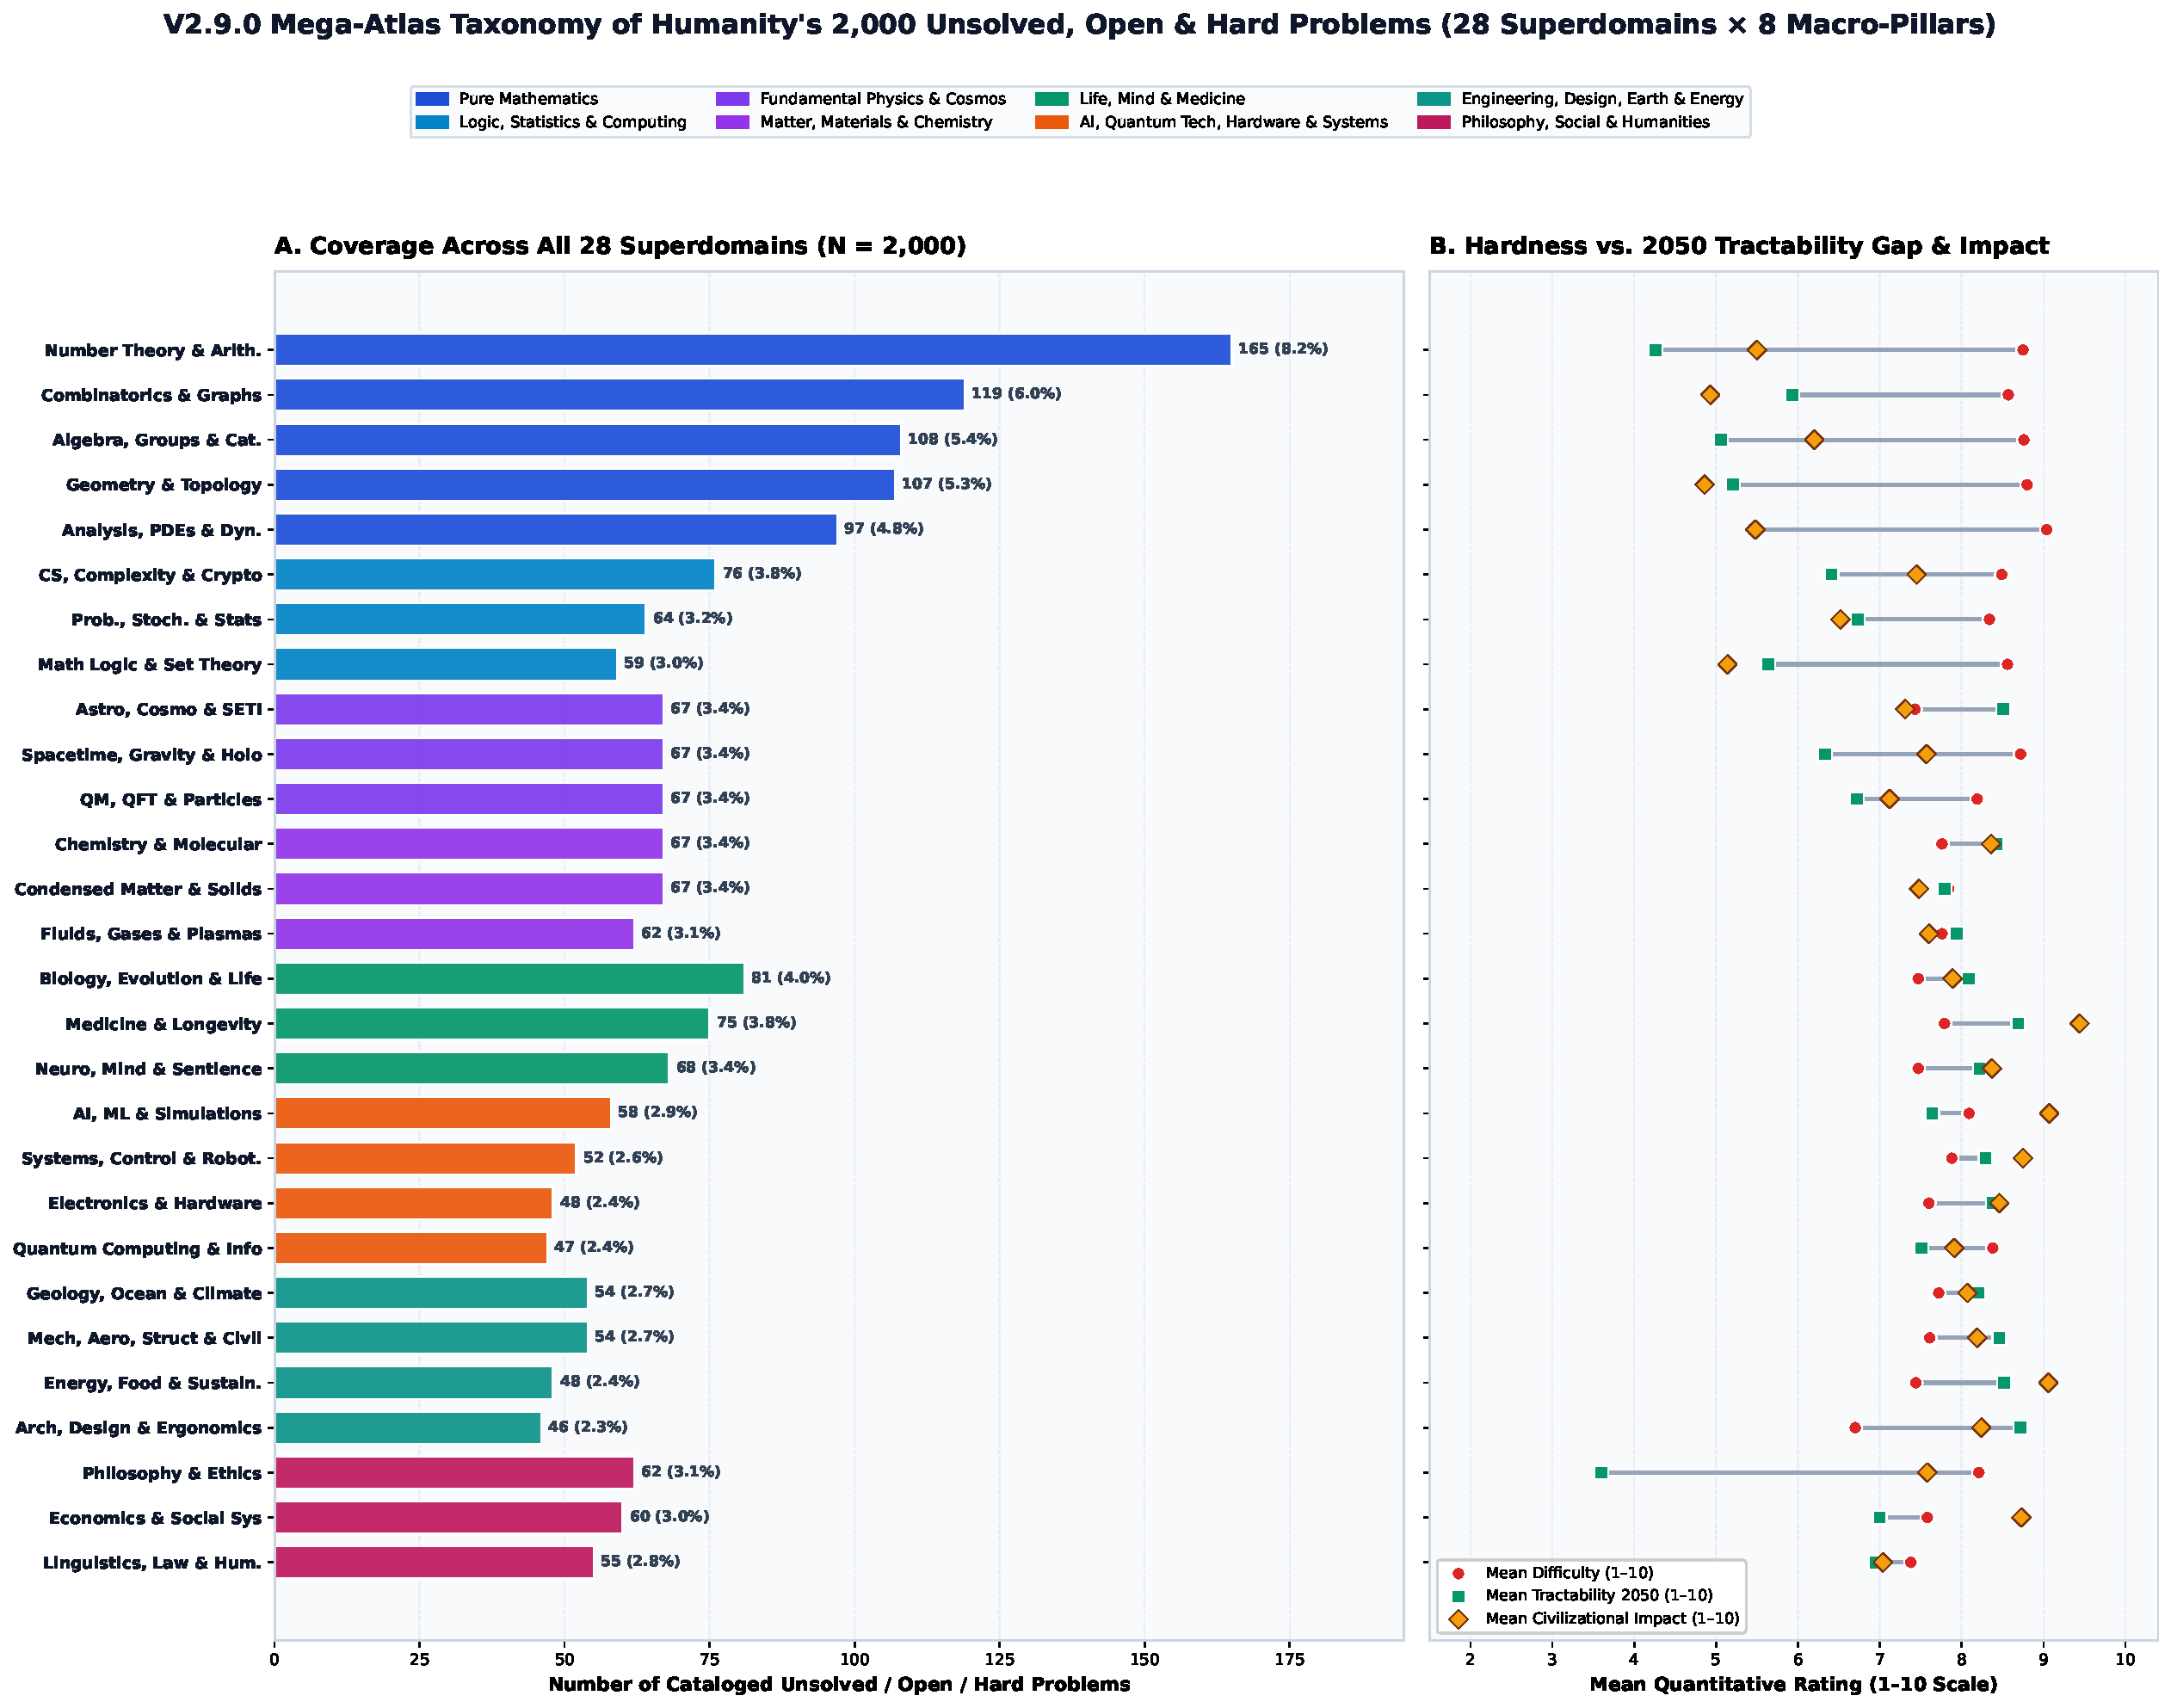
\includegraphics[width=0.90\textwidth]{figures/fig01_superdomain_landscape.pdf}
  \caption{Coverage across all $28$ Superdomains ($N=1{,}900$) alongside mean Difficulty, 2050 Tractability, and Civilizational Impact.}
  \label{fig:superdomains}
\end{figure}

\begin{figure}[p]
  \centering
  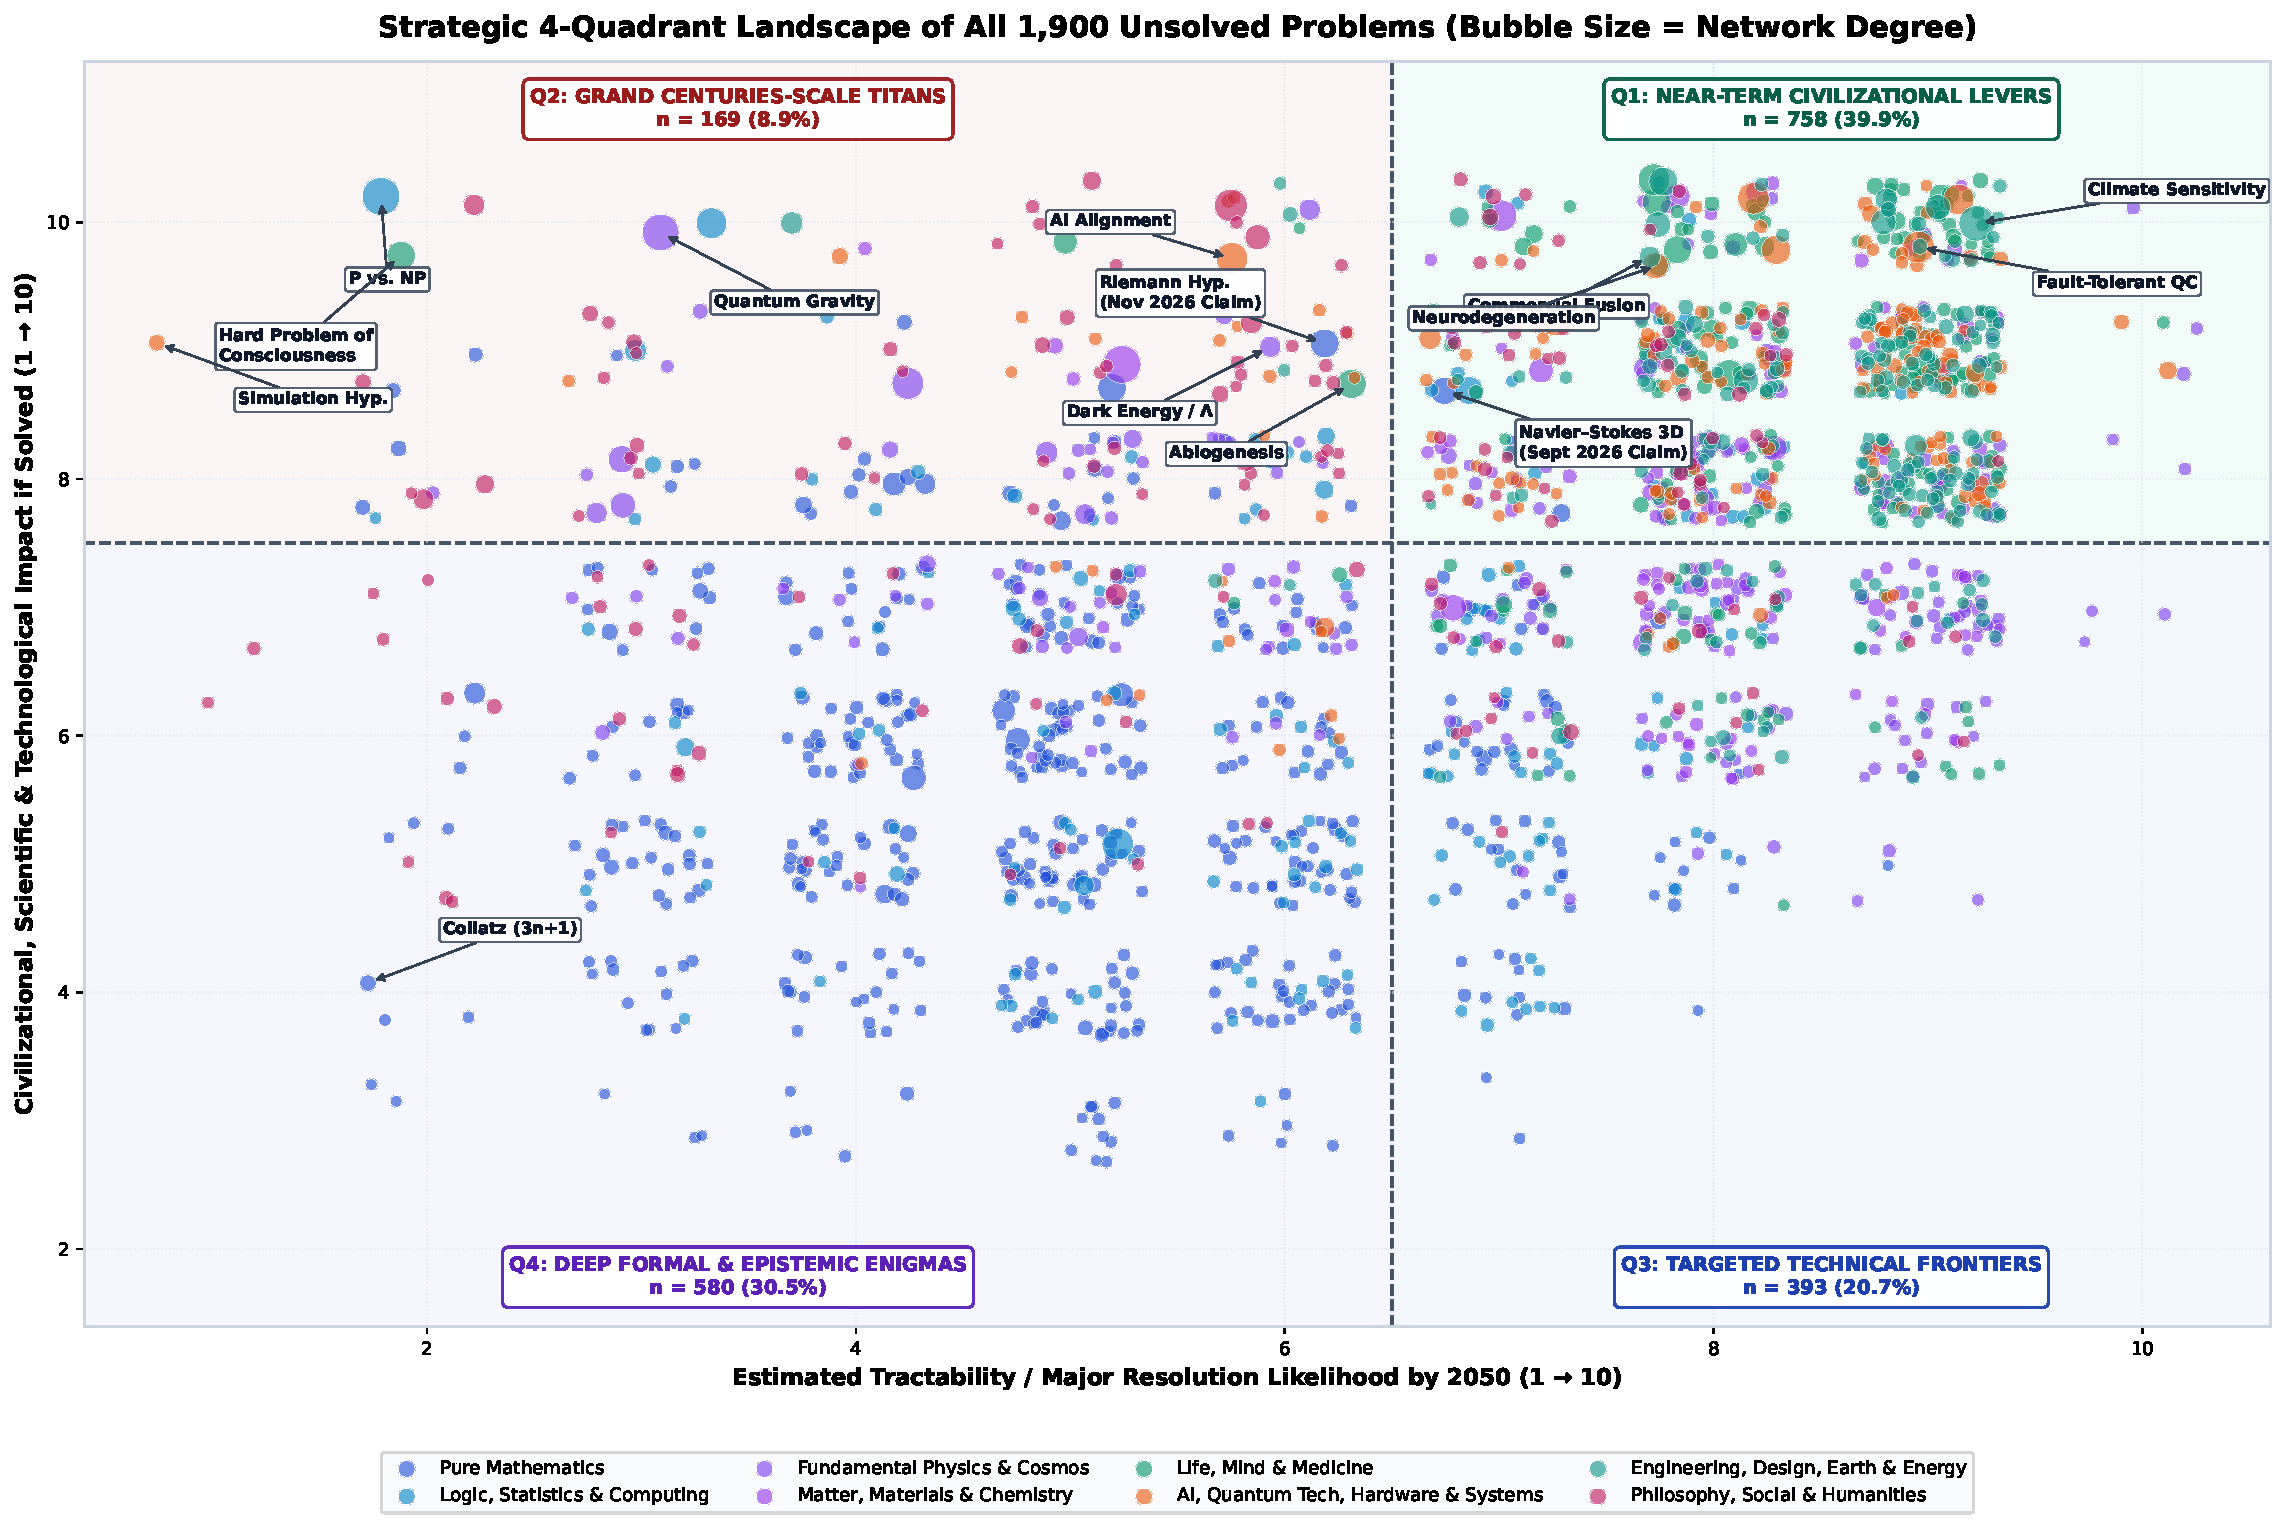
\includegraphics[width=0.90\textwidth]{figures/fig02_strategic_quadrant.pdf}
  \caption{Strategic 4-Quadrant landscape plotting Civilizational Impact against 2050 Tractability (bubble size proportional to network degree).}
  \label{fig:quadrant}
\end{figure}

\begin{figure}[t]
  \centering
  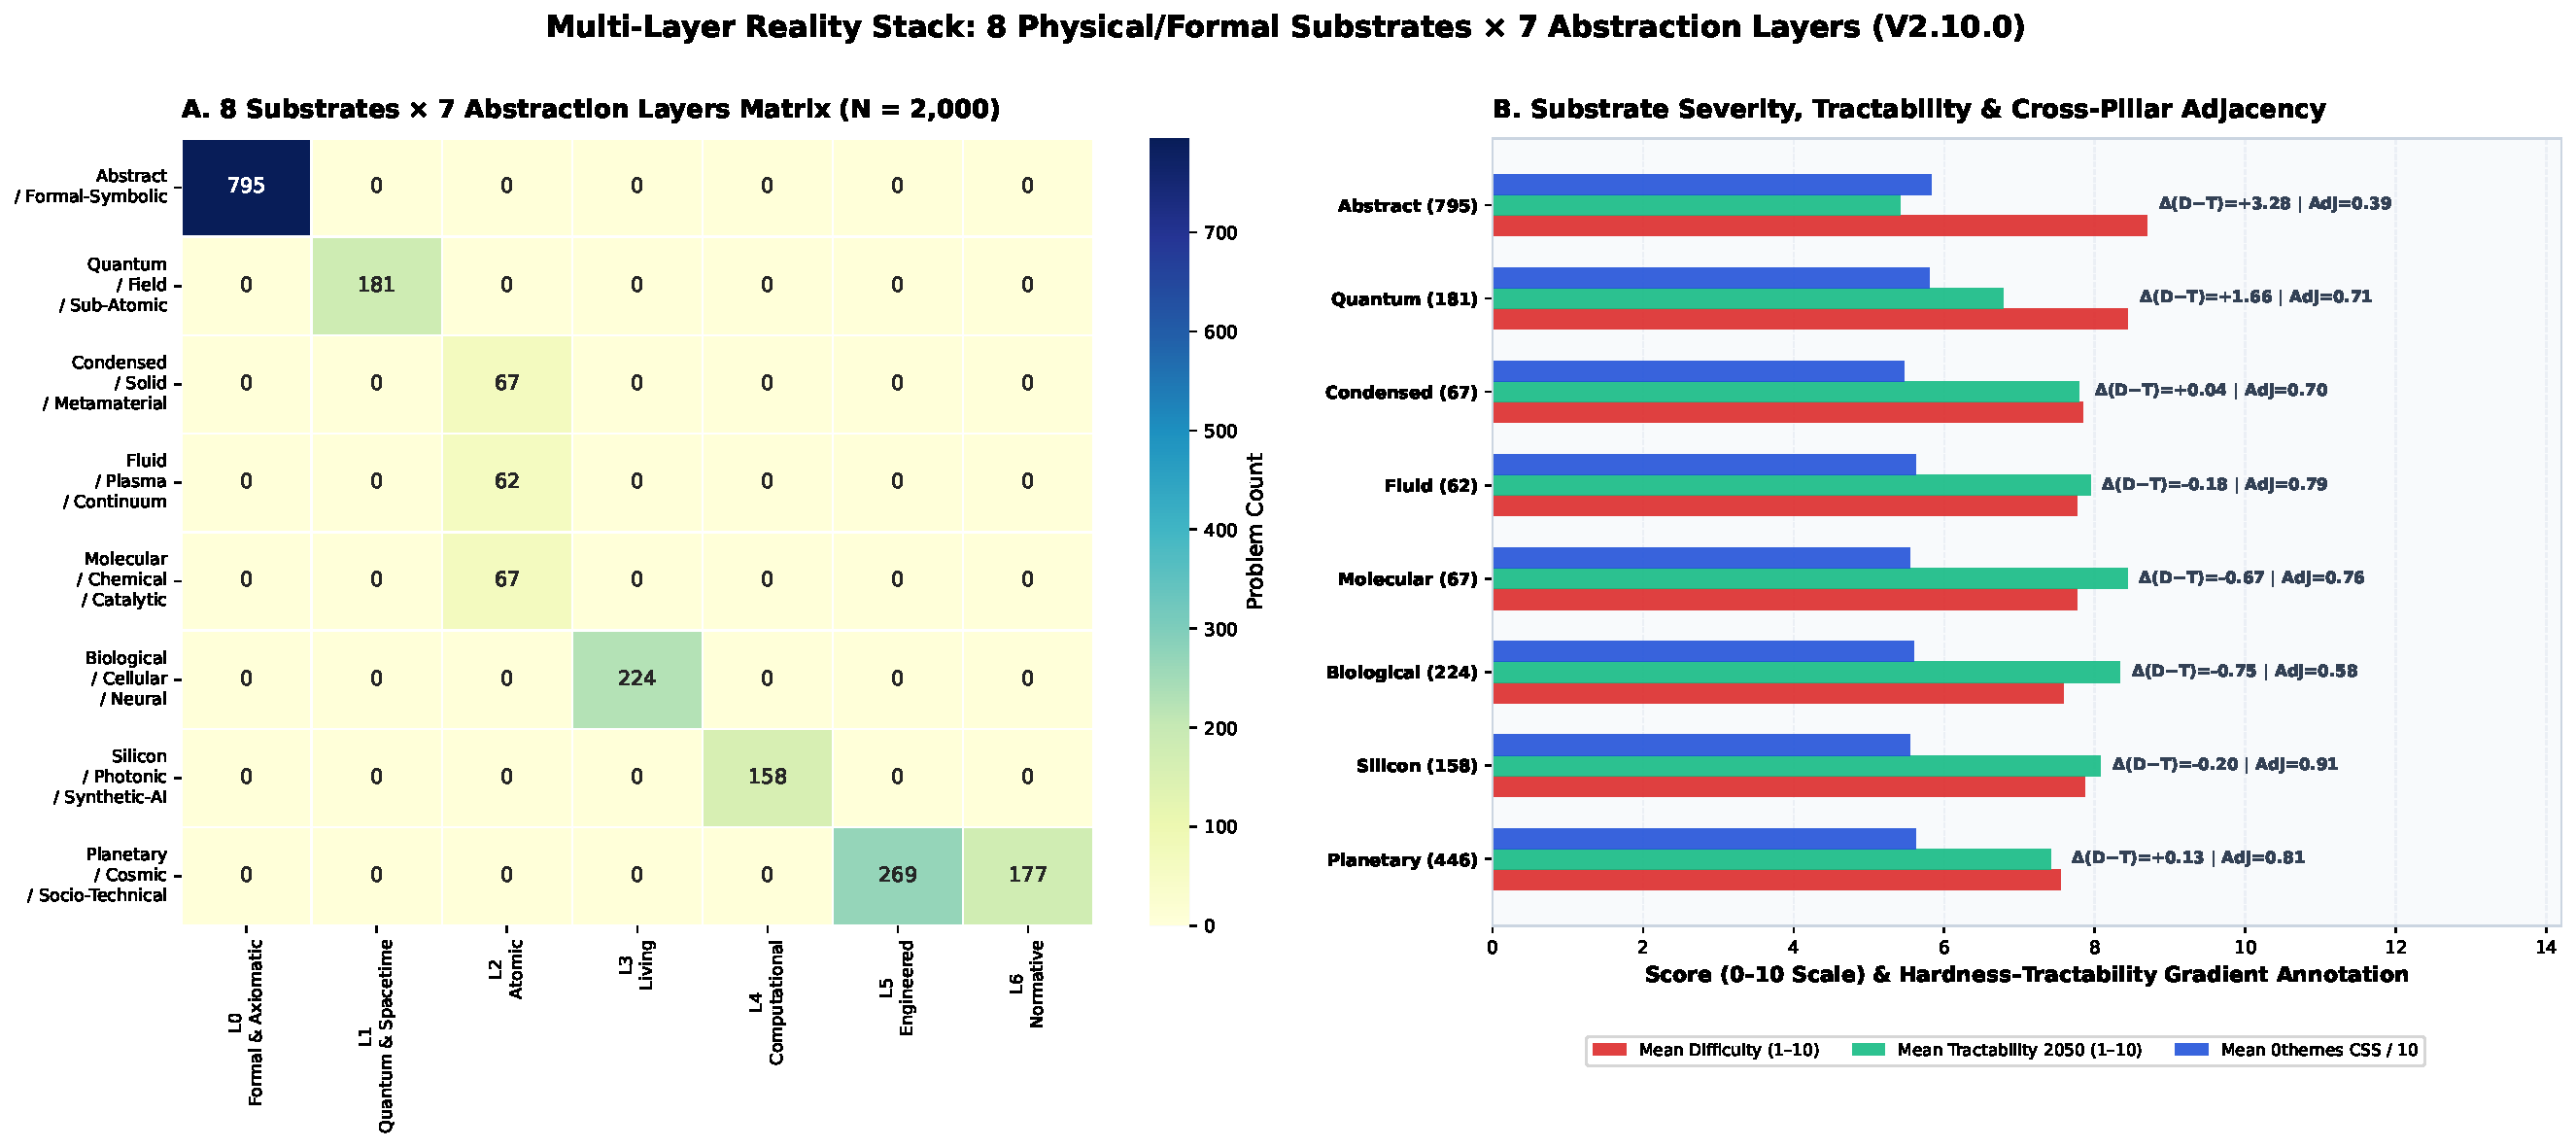
\includegraphics[width=0.95\textwidth]{figures/fig13_substrates_layers.pdf}
  \caption{Multi-Layer Reality Stack: $8$ Physical/Formal Substrates $\times$ $7$ Abstraction Layers ($\text{L0}$--$\text{L6}$) and mean hardness--tractability gradient $\Delta(D-T)$.}
  \label{fig:substrates}
\end{figure}

\subsection{Biconnected Knowledge Graph Analytics}
Graph topology is audited with NetworkX~\cite{hagberg2008networkx}: all $1{,}900$ nodes form $1$ connected component with $5{,}808$ undirected edges (mean degree $6.11$, $14$ modularity communities), $0$ articulation points, $0$ bridge edges (\code{nx.is_biconnected(G) == True}), and $0$ unresolved \code{raw_links}. Exactly $68$ problems qualify as \emph{Apex Multi-Pillar Keystones} (directly linked to $\ge 3$ distinct foreign Macro-Pillars), $239$ as \emph{Trans-Pillar Boundary Interfaces}, $1{,}108$ as \emph{Intra-Pillar Bridges}, and $485$ as \emph{Core Intra-Pillar Specialists}.

\section{Six-Kernel Pure Lean 4.35.0 Formalization and Statement-Fidelity Audit}
\label{sec:lean}

To eliminate silent formula drift, off-by-one threshold bugs, and reward-hacking regressions, we formalize all discrete structural invariants in zero-Mathlib \emph{Lean~4.35.0}~\cite{moura2021lean4} under strict compiler options (\code{autoImplicit = false}, \code{relaxedAutoImplicit = false}, \code{linter.unusedVariables = true}, \code{linter.deprecated = true}).

\subsection{Architecture and Six-Kernel Palomar Verification}
The Lean codebase comprises seven core modules (\code{Scoring}, \code{Quadrants}, \code{Taxonomy}, \code{GraphInvariants}, \code{AutoResearchInvariants}, \code{LayerGradients}, and \code{NonVacuity}) totaling $84$ base theorems, plus a clean challenge/solution boundary (\code{Challenge.lean}, \code{Solution.lean}, \code{PalomarSolution.lean}) matched against a \code{sorry}-only contract in \code{palomar/PalomarChallenge.lean} via \code{lake comparator --config comparator.json --paranoid}. Every one of the $92$ audited theorems in \code{MegaAtlasProofs/VerifyAxioms.lean} compiles with $0$ \code{sorry} in \code{lean/}, $0$ \code{native_decide}, $0$ custom axioms, and depends strictly on constructive axioms within [\code{propext}, \code{Quot.sound}] (no \code{Classical.choice}). All exported terms ($1{,}753$ declarations) pass six independent proof checkers: Lean~4.35.0's default kernel, \code{leanchecker-paranoid}, \code{lean4lean}, \code{nanoda_bin}, \code{con-leche --verified}, and \code{con-ron --verified}.

\subsection{Non-Vacuity Witnesses and Statement-Fidelity Matrix}
A formal theorem of the form $H \to C$ can hold vacuously if $H$ is unsatisfiable. Module \code{MegaAtlasProofs.NonVacuity} ($12$ theorems) therefore constructs explicit concrete inhabitants for \emph{every} hypothesis bundle---including valid CSS/Titan ratings, the sharp non-saturation boundary at $299$ years (\code{ageScoreCentis 299 < 10000}), all $4$ Quadrants, all $6$ Eras, a concrete $3$-vertex cross-pillar simple triangle inhabiting the Handshaking Lemma, strict deduplication shrinkage, concrete AutoResearch keep/discard traces mirroring \code{autoresearch/results.tsv}, and all $4$ MarginRole classes at the exact $30\%$ ($3000$\,bps) boundary.

Table~\ref{tab:fidelity} documents the exact correspondence and intentional scope boundaries between the paper/Python definitions and their Lean~4.35.0 formalizations (full 18-row table in \code{docs/statement-fidelity.md}).

\begin{table}[t]
\centering
\caption{Statement-Fidelity Audit Matrix mapping Python runtime definitions to Lean 4.35.0 formalizations and noting exact scope boundaries.}
\label{tab:fidelity}
\scriptsize
\renewcommand{\arraystretch}{1.16}
\begin{tabularx}{\textwidth}{@{}P{0.62cm}P{2.25cm}YP{3.2cm}P{2.7cm}@{}}
\toprule
\textbf{Grp} & \textbf{Lean Target} & \textbf{Formalized Property} & \textbf{Python Implementation} & \textbf{Scope Divergence} \\
\midrule
M1 & \tcode{Scoring.lean} ($22$ thms) & Exact integer bps/centi bounds, weights sum to $100$, monotonicity, $300$-yr age cap. & \tcode{compute_css_score}, \tcode{titan_index} & $\ln(1+\deg)$ abstracted as bounded input; checked differentially vs.\ 50-digit \tcode{Decimal} oracle. \\
M2 & \tcode{Quadrants.lean} ($11$ thms) & Exact iff for Q1--Q4, $\mathrm{Q1} \Rightarrow \mathrm{Lev} \ge 5.6$, monotone $6$-Era partition. & \tcode{classify_quadrant}, \tcode{compute_era} & Exact $1$-to-$1$ isomorphism (zero divergence). \\
M3 & \tcode{Taxonomy.lean} ($8$ thms) & $8$ Pillars, $28$ SDs, $[5,3,3,3,3,4,4,3]$ partition, surjectivity, cross-pillar $\Rightarrow$ cross-SD. & \tcode{MACRO_PILLARS}, \tcode{SUPERDOMAIN_TO_PILLAR} & Exact $1$-to-$1$ isomorphism. \\
M4 & \tcode{GraphInvariants} ($5$ thms) & Handshaking $\sum \deg = 2|E|$, cross-pillar $\le$ cross-SD $\le |E|$, $|\mathrm{dedup}(x)| \le |x|$. & \tcode{nx.Graph}, \tcode{load_v2_master} & Biconnectivity ($0$ APs, $0$ bridges) audited programmatically via NetworkX. \\
M5 & \tcode{AutoResearchInv.} ($12$ thms) & \tcode{aqsBps} bounds, anti-gaming (\tcode{gates=false} $\Rightarrow$ discard), monotone ratchet, delta antisymmetry. & \tcode{autoresearch/evaluate.py}, \tcode{compare_two_problems} & Exact $1$-to-$1$ integer basis-point correspondence. \\
M6 & \tcode{LayerGradients} ($14$ thms) & $8$ Substrates, $7$ Layers, $D-T \in [-9,9]$, bridge ratio $\le 100\%$, $4$-class \tcode{MarginRole}. & \tcode{classify_margin_role}, \tcode{SUBSTRATE_CLASSES} & Exact $1$-to-$1$ correspondence (bps = $\lfloor 10^4 r \rfloor$). \\
M7 & \tcode{NonVacuity.lean} ($12$ thms) & Concrete inhabitants + sharp negative boundaries for all hypotheses M1--M6. & \tcode{tests/test_properties_and_differential.py} & Zero vacuous theorems across all $92$ entries. \\
\bottomrule
\end{tabularx}
\end{table}

\section{Hybrid RAG, 10-Tool MCP Server, AutoResearch, and Track B Pilot}
\label{sec:rag_ar}

To enable deterministic, zero-API-key programmatic consumption, \code{rag/query.py} indexes all $1{,}900$ records in a Porter-stemmed SQLite FTS5 database (auto-built on demand on fresh git clones) and executes a staged retrieval pipeline: exact-ID shortcut $\to$ exact-phrase FTS5 $\to$ strict-AND FTS5 $\to$ relaxed-OR backfill $\to$ hybrid re-ranking combining normalized BM25 ($0.22$), title token coverage ($0.24$), contiguous title-bigram coverage ($0.18$), body coverage ($0.10$), NetworkX degree/PageRank graph authority ($0.23$), and CSS prior ($0.03$). On the immutable $25$-query cross-pillar Gold Benchmark inside \code{autoresearch/evaluate.py}, this ratchet raised RAG MRR@5 from $82.22\%$ ($19/25$ top-1) to $100.0\%$ ($25/25$ top-1) at $< 10$\,ms median query latency, raising the immutable Atlas Quality Score (\code{AQS}) from $91.69$ to $97.99$ while transparently logging discarded hypotheses (\code{H-002}, \code{H-004}) in \code{autoresearch/results.tsv} (Figure~\ref{fig:autoresearch}), inspired by Karpathy's AutoResearch pattern~\cite{karpathy2026autoresearch}.

\begin{figure}[t]
  \centering
  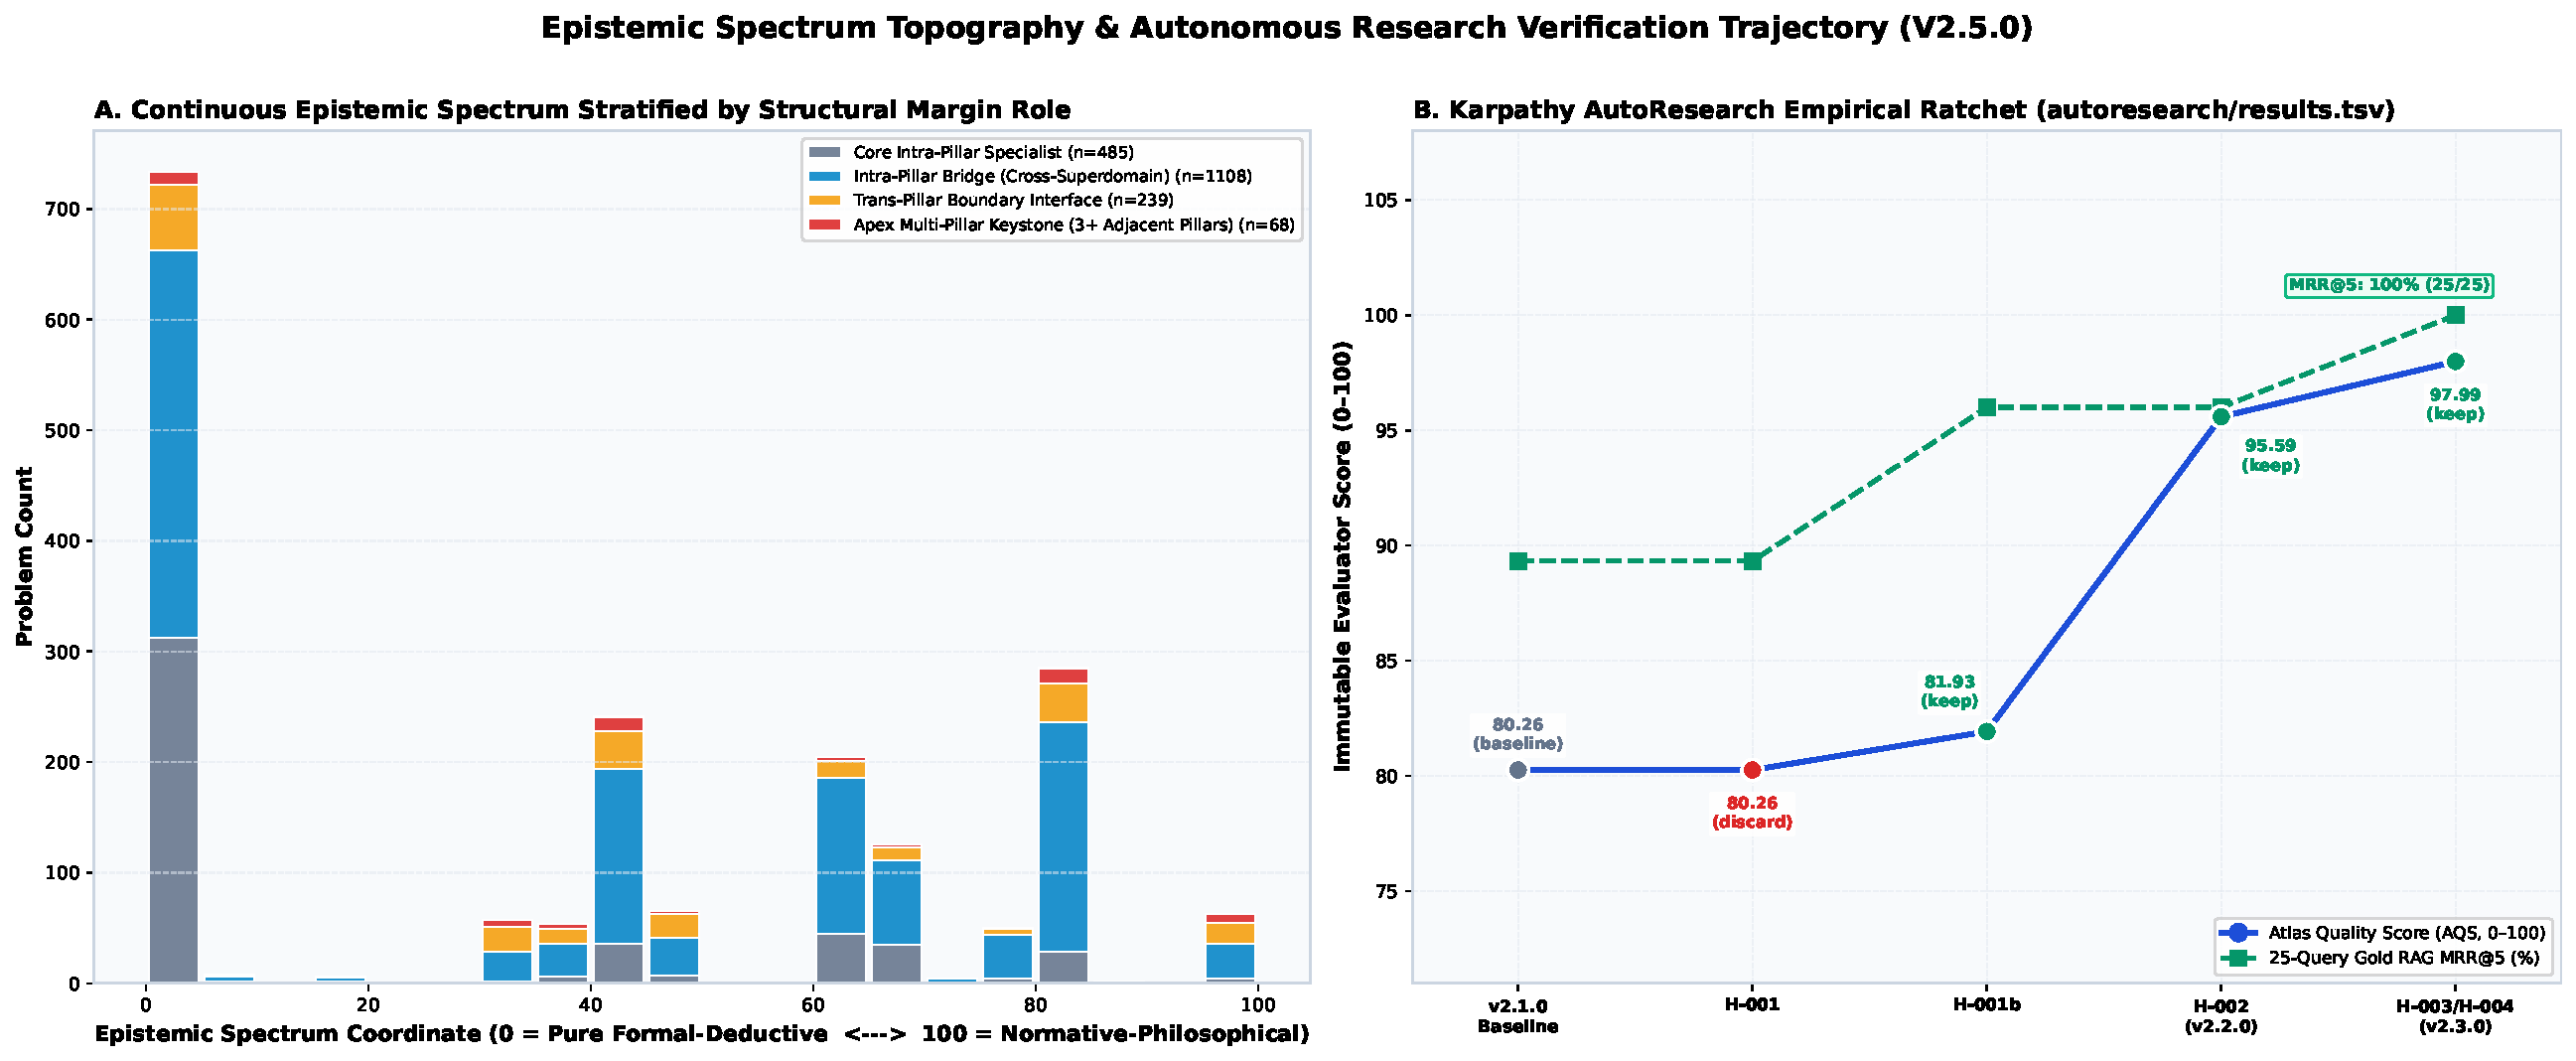
\includegraphics[width=0.95\textwidth]{figures/fig15_spectrum_autoresearch.pdf}
  \caption{Continuous Epistemic Spectrum stratified by Margin Role (left) and the immutable AutoResearch empirical ratchet across logged kept and discarded hypotheses (right).}
  \label{fig:autoresearch}
\end{figure}

The zero-dependency stdio JSON-RPC~2.0 server (\code{mcp_server/server.py}) speaks both NDJSON and \code{Content-Length:} LSP/MCP framing and exposes $10$ grounded tools (\code{search_problems}, \code{get_problem}, \code{compare_problems}, \code{list_nov2026_ai_claims}, \code{get_top_ranked}, \code{get_pillar_summary}, \code{get_substrate_layer_summary}, \code{get_margin_and_gradient_extremes}, \code{list_author_frontier_contributions}, and \code{get_atlas_provenance}). As a reproducible Track~B demonstration, \code{research/runs/LOG-002_antihydra_pilot/antihydra_probe.py} executes $5{,}000$ exact arbitrary-precision steps of the Busy Beaver $BB(6)$ Antihydra recurrence ($a_0=8, b_0=0$: non-halting through step $5{,}000$, $b_{5000}=2{,}599$, $\min b = 0$, empirical drift $+0.5198$/step) plus a $99$-seed perturbation sweep ($a_0 \in [2,100]$, $66$ halting, $33$ surviving to $2{,}000$ steps), explicitly affirming that \code{LOG-002} remains \textbf{OPEN}.

\section{Author-Curated Scoped Frontier Preprints (Non-Retirement Audit)}
\label{sec:author_preprints}

To answer whether any cataloged Mega-Atlas problems have been solved in companion repositories maintained in \code{0thernes-research-archive}~\cite{donahue2026archive}, Table~\ref{tab:author_preprints} cross-maps all seven machine-checked independent preprints against their parent Atlas IDs. \emph{Conflict-of-interest and scope notice:} these are self-authored independent preprints (not externally peer-reviewed) that resolve narrowly scoped published sub-conjectures or establish formal structural invariants. Every overarching Mega-Atlas parent problem remains explicitly \textbf{OPEN} ($0 / 1{,}900$ retired).

\begin{table}[t]
\centering
\caption{Cross-map of companion author preprints in \code{0thernes-research-archive}~\cite{donahue2026archive} against parent Mega-Atlas IDs. All overarching Atlas parents remain \textbf{OPEN}; preprints are self-published and not externally peer-reviewed.}
\label{tab:author_preprints}
\scriptsize
\renewcommand{\arraystretch}{1.16}
\begin{tabularx}{\textwidth}{@{}P{2.05cm}P{2.25cm}P{2.25cm}YP{1.2cm}@{}}
\toprule
\textbf{Archive ID} & \textbf{Parent IDs} & \textbf{Verification} & \textbf{Narrowly Scoped Result} & \textbf{Parent} \\
\midrule
\tcode{0TH-2026-012} & \tcode{CS-053}, \tcode{CS-026}, \tcode{CS-001}, \tcode{CS-051} & Lean 4.35 ($6/6$ kernels) & Koszul--Veronese syzygy rank ($4/7 \to 10/17$), LFSR domination, Chen Step~9 DFT cancellation, $8/13$ polymatroid, $\mathbb{F}_{11}$ Byzantine witness. & \textbf{OPEN} \\
\tcode{0TH-2026-011} & $13$ Crypto/QC IDs & Lean 4.35 ($6/6$ kernels) & $27$ algebraic/IT/QGT invariants incl.\ $c_{\mathrm{eff}}^2+C^2=1$ and sharp FIPS~203 $|e|\le 831$. & \textbf{OPEN} \\
\tcode{0TH-2026-010} & \tcode{CS-005} & Lean 4.35 ($7$ kernels)~\cite{donahue2026catalytic} & Base-$p$ $2$-register passive catalytic dichotomy and unique optimal $3$-register exponent $\log_{13} 8 \approx 0.8107$. & \textbf{OPEN} \\
\tcode{0TH-2026-009} & \tcode{QM-011} & Lean 4.35 / Mathlib ($6/6$) & Jonah Conjecture~E ($9$ vertex cases, $N \ge 4$), disjoint Mermin formulas $(7^k-5^k)/2$, $4$-qubit $C_3$ optima. & \textbf{OPEN} \\
\tcode{0TH-2026-004} & \tcode{QM-011} & Lean 4.35 ($6/6$) + DRUP & Exact minimum KS ray counts inside restricted pools ($31, 33, 18, 29$). & \textbf{OPEN} \\
\tcode{0TH-2026-006} & \tcode{STAT-001} (rel.) & Lean 4.35 / Mathlib & Resolved Bani\'c--Elezovi\'c Conjecture~7.7 ($a_{\triangle} = 1/32 - 4\sqrt{3}/243$); standalone sub-conjecture. & \textbf{N/A} \\
\tcode{0TH-2026-007/8} & \tcode{NEURO-001}, \tcode{NEURO-019} & Lean 4.35 ($6/6$)~\cite{donahue2026synapse} & $18$ biophysical invariants + refuted pre-registered $40$\,Hz ATP sustainability ($f_{\mathrm{crit}}=29.5625$\,Hz). & \textbf{OPEN} \\
\bottomrule
\end{tabularx}
\end{table}

\section{Threats to Validity, Limitations, and Falsifiability}
\label{sec:limitations}

\begin{enumerate}[leftmargin=1.5em]
  \item \textbf{Editorial Score Subjectivity:} The $1$--$10$ inputs ($d, t, i, r$) are curated AI-assisted editorial estimates, not inter-rater psychometric surveys. Because the source modules in \code{src/v2_data/} and the deterministic rebuild pipeline are public, any researcher can edit scores, re-run \code{just reproduce}, and inspect exact rank diffs.
  \item \textbf{Registry Coverage Skew:} Pure Mathematics ($27.1\%$) has denser historical registries than applied engineering or humanities; $952$ records are explicitly flagged \code{ai-assisted-editorial-synthesis} rather than \code{primary-registry-indexed}.
  \item \textbf{Formal vs.\ Runtime Scope:} Lean~4.35.0 certifies integer basis-point formulas over bounded inputs; IEEE-754 \code{log1p} terms are differentially audited against our $50$-digit \code{Decimal} oracle in \code{reference/scoring_oracle.py} rather than inside Lean.
  \item \textbf{No External Peer Review:} Neither this dataset nor this white paper has undergone journal peer review. All FAIR descriptors follow Gebru et al.~\cite{gebru2021datasheets}, MLCommons Croissant~1.0~\cite{akhtar2024croissant}, and RO-Crate~1.1~\cite{soilandreyes2022rocrate} so independent referees can audit every file byte-for-byte.
\end{enumerate}

\section{Reproducibility, AI-Assistance Disclosure, CRediT, and Availability}
\label{sec:repro}

\subsection{One-Command Reproduction}
On a clean clone with Python~3.12, Lean~4.35.0 (\code{elan}), and Tectonic installed:
\begin{verbatim}
just setup && just reproduce && just test && just lean && just paper
\end{verbatim}
Every GitHub push to \code{main} runs a $3$-OS Python matrix (Ubuntu, macOS, Windows), the $6$-kernel Lean~4.35.0 Palomar comparator inside a \code{bubblewrap} sandbox, Tectonic AMS-LaTeX + clean-room \code{arxiv_submission.tar.gz} verification, SHA-256 manifest checks, and SLSA build-provenance attestation (\code{actions/attest-build-provenance@v2}). Full clean-clone replication logs are recorded in \code{REPLICATION.md}.

\subsection{AI-Assistance Disclosure, CRediT Authorship, and COI}
\textbf{Authorship \& CRediT:} Alexander Stephen Donahue (Independent Researcher, Spokane, WA, USA; ORCID \code{0009-0006-8168-9648}) is the sole human author responsible for Conceptualization, Methodology, Formal Audit Direction, Validation, Supervision, and Writing---Review \& Editing. \textbf{Disclosed AI Assistance:} Large language model coding and research agents (\code{Gemini / Antigravity}) assisted with Python pipeline engineering, Lean~4.35.0 tactic proofs, test/oracle authoring, figure generation, and manuscript drafting under direct human supervision and multi-cycle adversarial auditing (see \code{docs/AI_DISCLOSURE.md} and \code{lean/formalization.yaml}). \textbf{Conflict of Interest:} Section~\ref{sec:author_preprints} references seven companion preprints authored by A.\,S.~Donahue; none are counted as retiring any overarching Mega-Atlas problem.

\subsection{Data, Code, and Archival Availability}
All source code, Lean~4.35.0 proofs, tests, and scripts are licensed under \textbf{Apache-2.0}; all datasets, figures, documentation, and this manuscript are licensed under \textbf{CC-BY-4.0}.
\begin{itemize}[leftmargin=1.5em]
  \item \textbf{Canonical Repository:} \url{https://github.com/0thernes/unsolved-problems-mega-atlas}
  \item \textbf{Interactive Web Atlas \& Lean Proof Blueprint:} \url{https://0thernes.github.io/unsolved-problems-mega-atlas/}
  \item \textbf{Frozen Master Archive (\code{0TH-BUILD-007}):} \url{https://github.com/0thernes/0thernes-research-archive}
\end{itemize}

\FloatBarrier
\bibliographystyle{amsplain}
\bibliography{refs}

\end{document}
